\chapter{音響エネルギ分布特性}
Strength$G$、話声に対応する明瞭度$D_{50}$、音楽に対応する明瞭度である初期/後期反射音エネルギ比$C_{80}$、初期残響時間$EDT$、初期側方反射エネルギ率$LF$、両耳間相互相関度$IACC$を算出した。
(A)矩形モデルにおける各種音響物理指標の平面コンター図、度数分布表、各指標値と音源-観測点間距離$r$[m]の関係を以下に示す。
なお、音源はコンター図内(x,y,z)=(0,8,2.5)に位置し、ステージ先端はy=10にあたる(\figref{zahyo})。度数分布表内の破線は各観測高さ内にある105の観測点の平均値$\mu$を表す。

\begin{figure}[htbp]
    \centering
    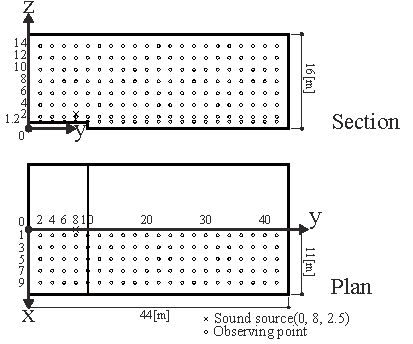
\includegraphics[keepaspectratio,scale=1]{04_att/zahyo.pdf}
    \caption{\hspace{1mm}Rectangular coordinate system of model}
    \label{fig:zahyo}
\end{figure}

\newpage
      \begin{minipage}{1\textwidth}
        \centering
          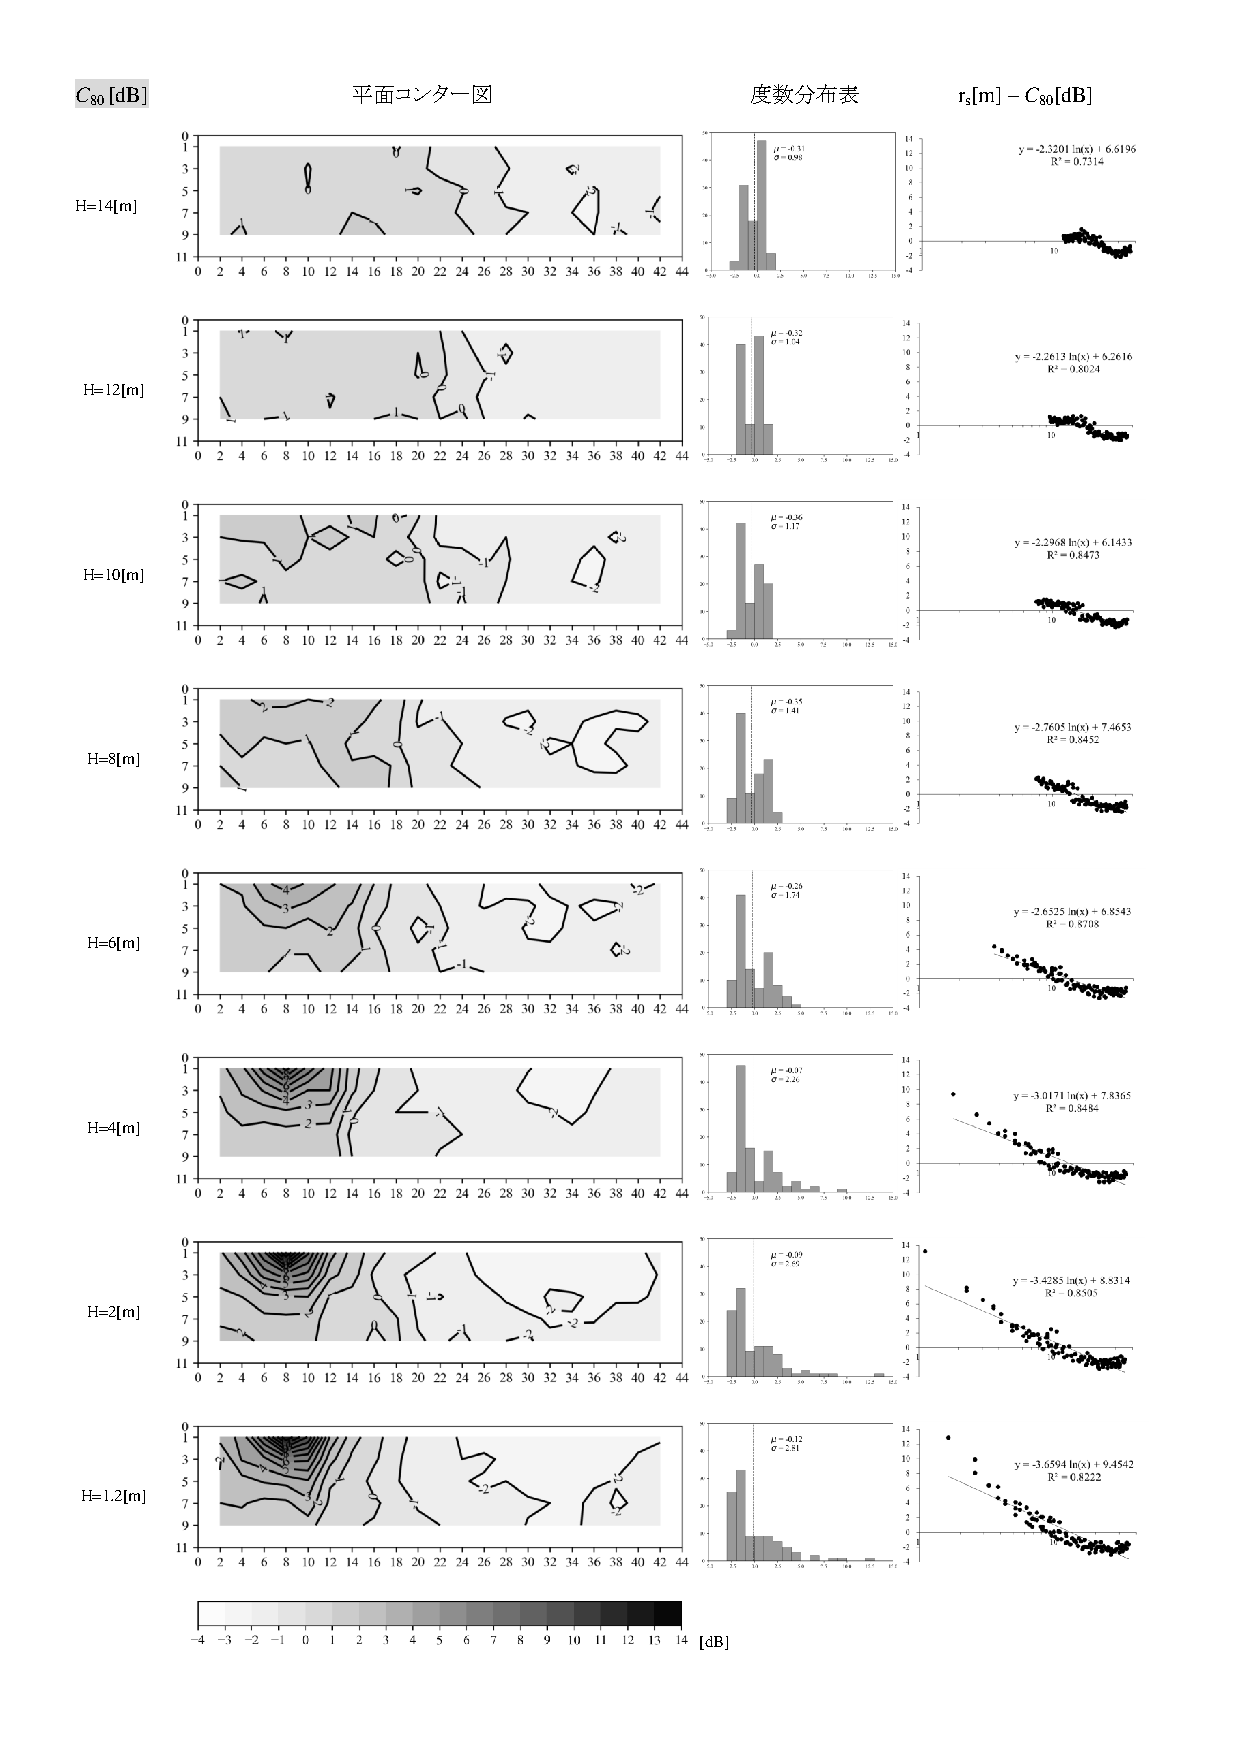
\includegraphics[keepaspectratio,width=1\hsize,angle=0]
                          {04_att/Onkyo_rec1.pdf}
      \end{minipage}
\newpage
      \begin{minipage}{1\textwidth}
        \centering
          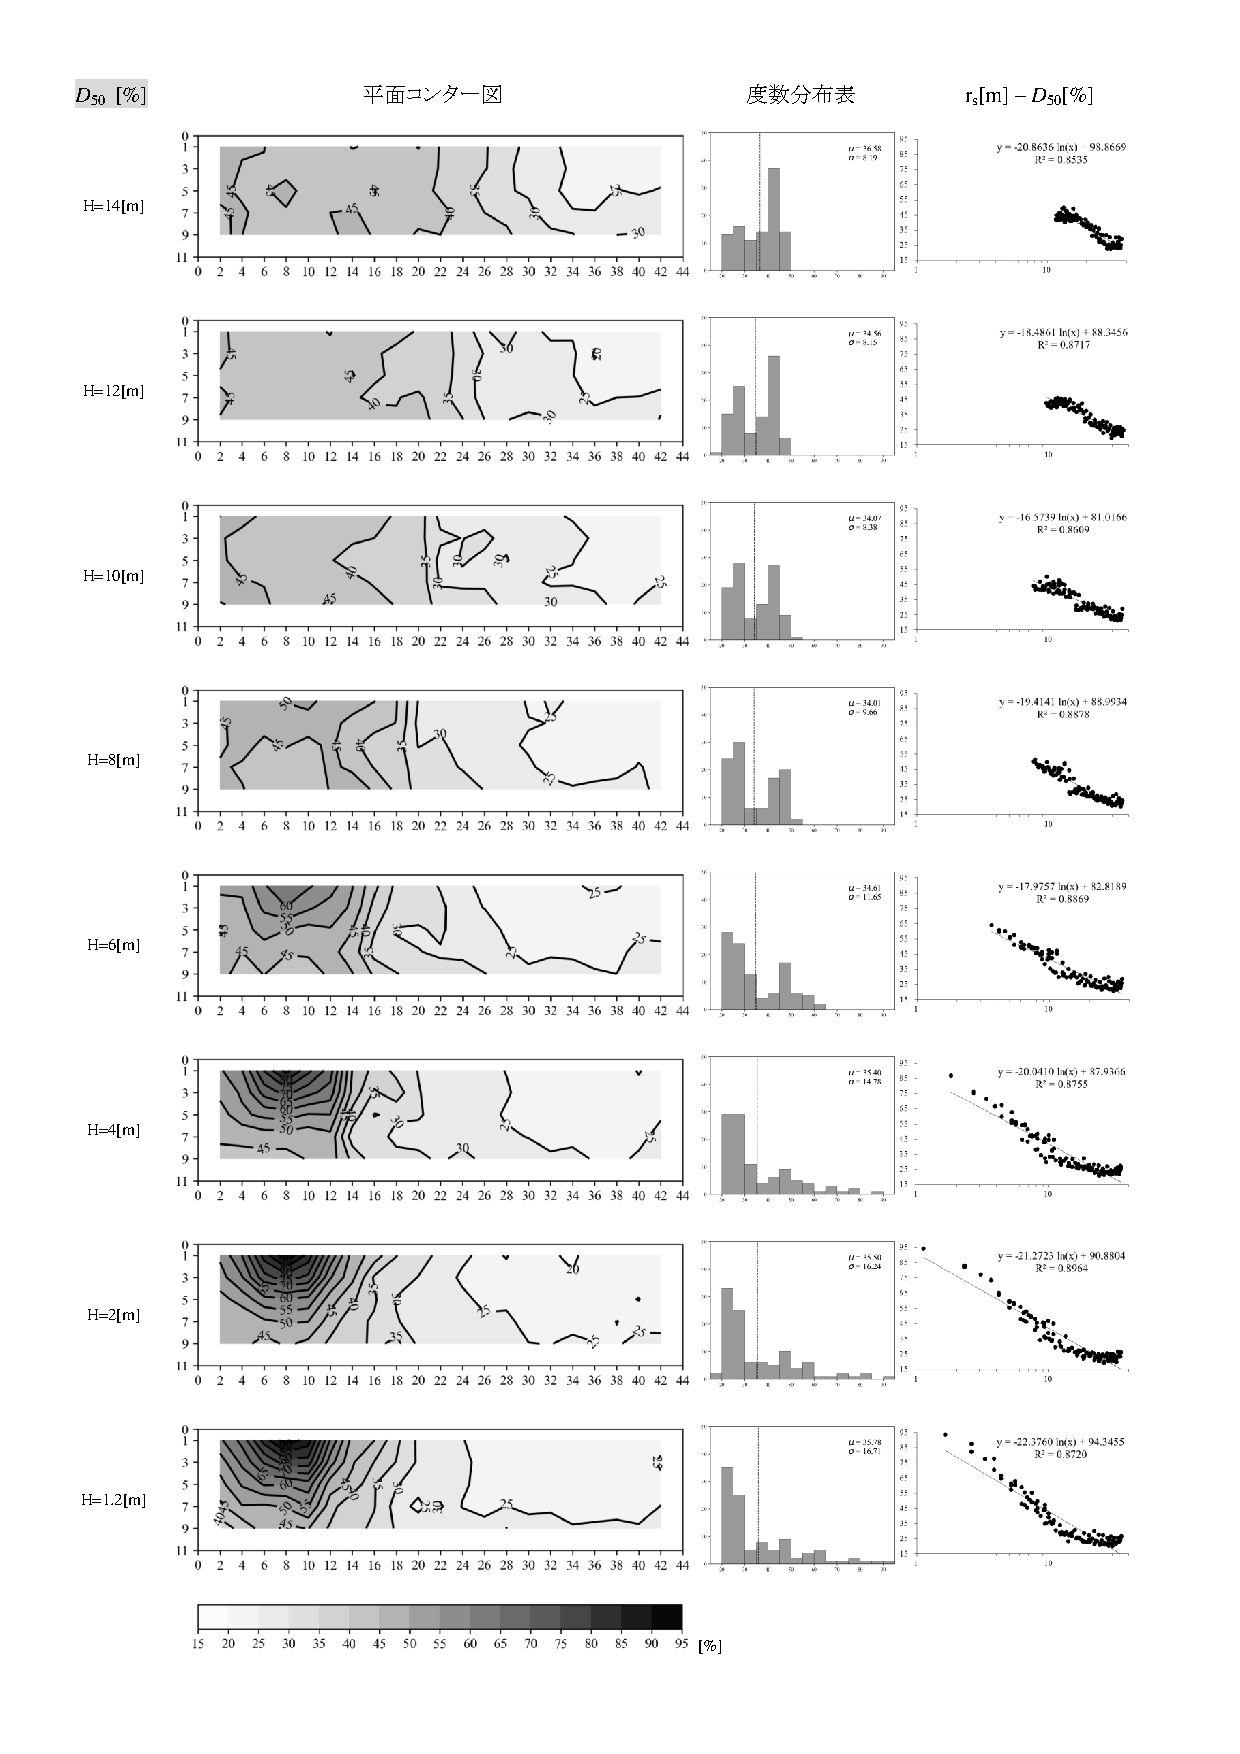
\includegraphics[keepaspectratio,width=1\hsize,angle=0]
                          {04_att/Onkyo_rec2.pdf}
      \end{minipage}
\newpage
      \begin{minipage}{1\hsize}
        \centering
          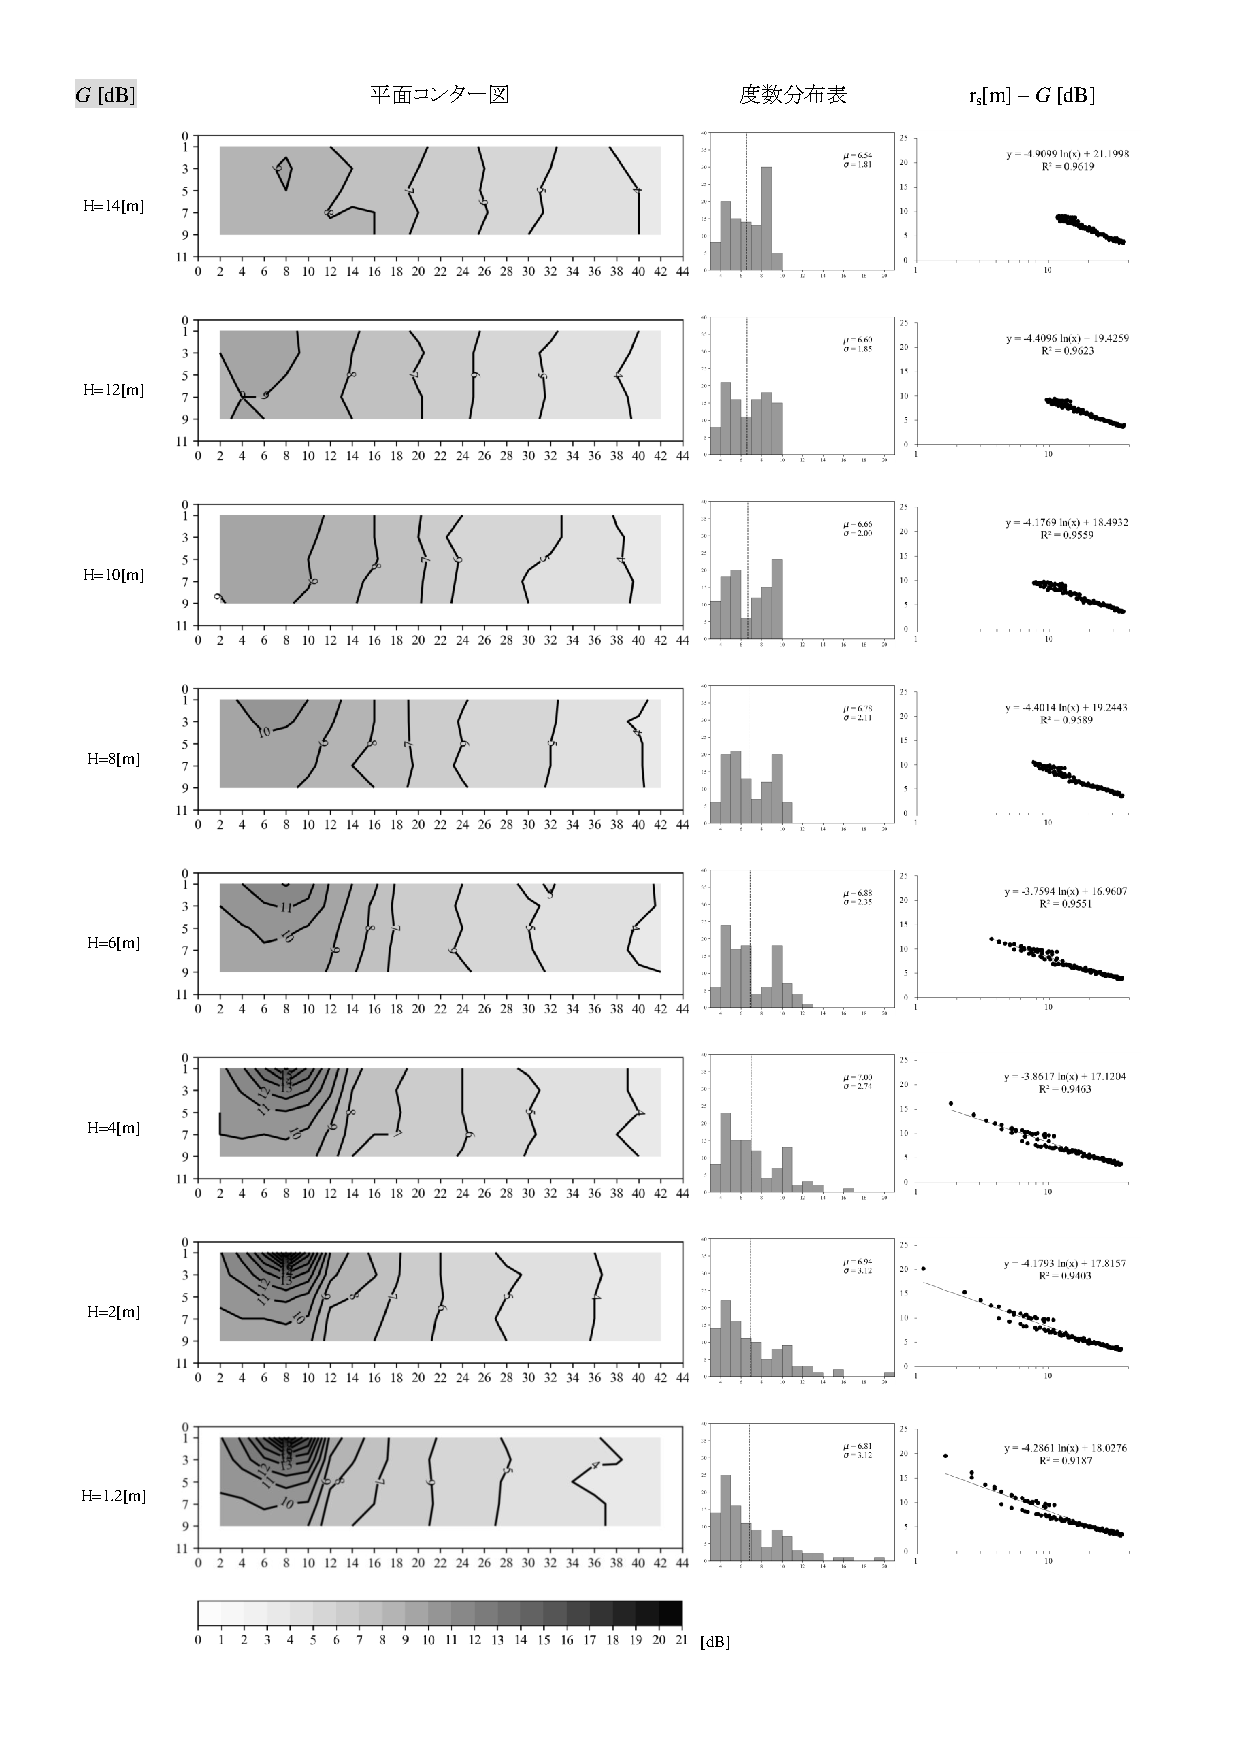
\includegraphics[keepaspectratio,width=1\hsize,angle=0]
                          {04_att/Onkyo_rec3.pdf}
      \end{minipage}
\newpage
      \begin{minipage}{1\hsize}
        \centering
          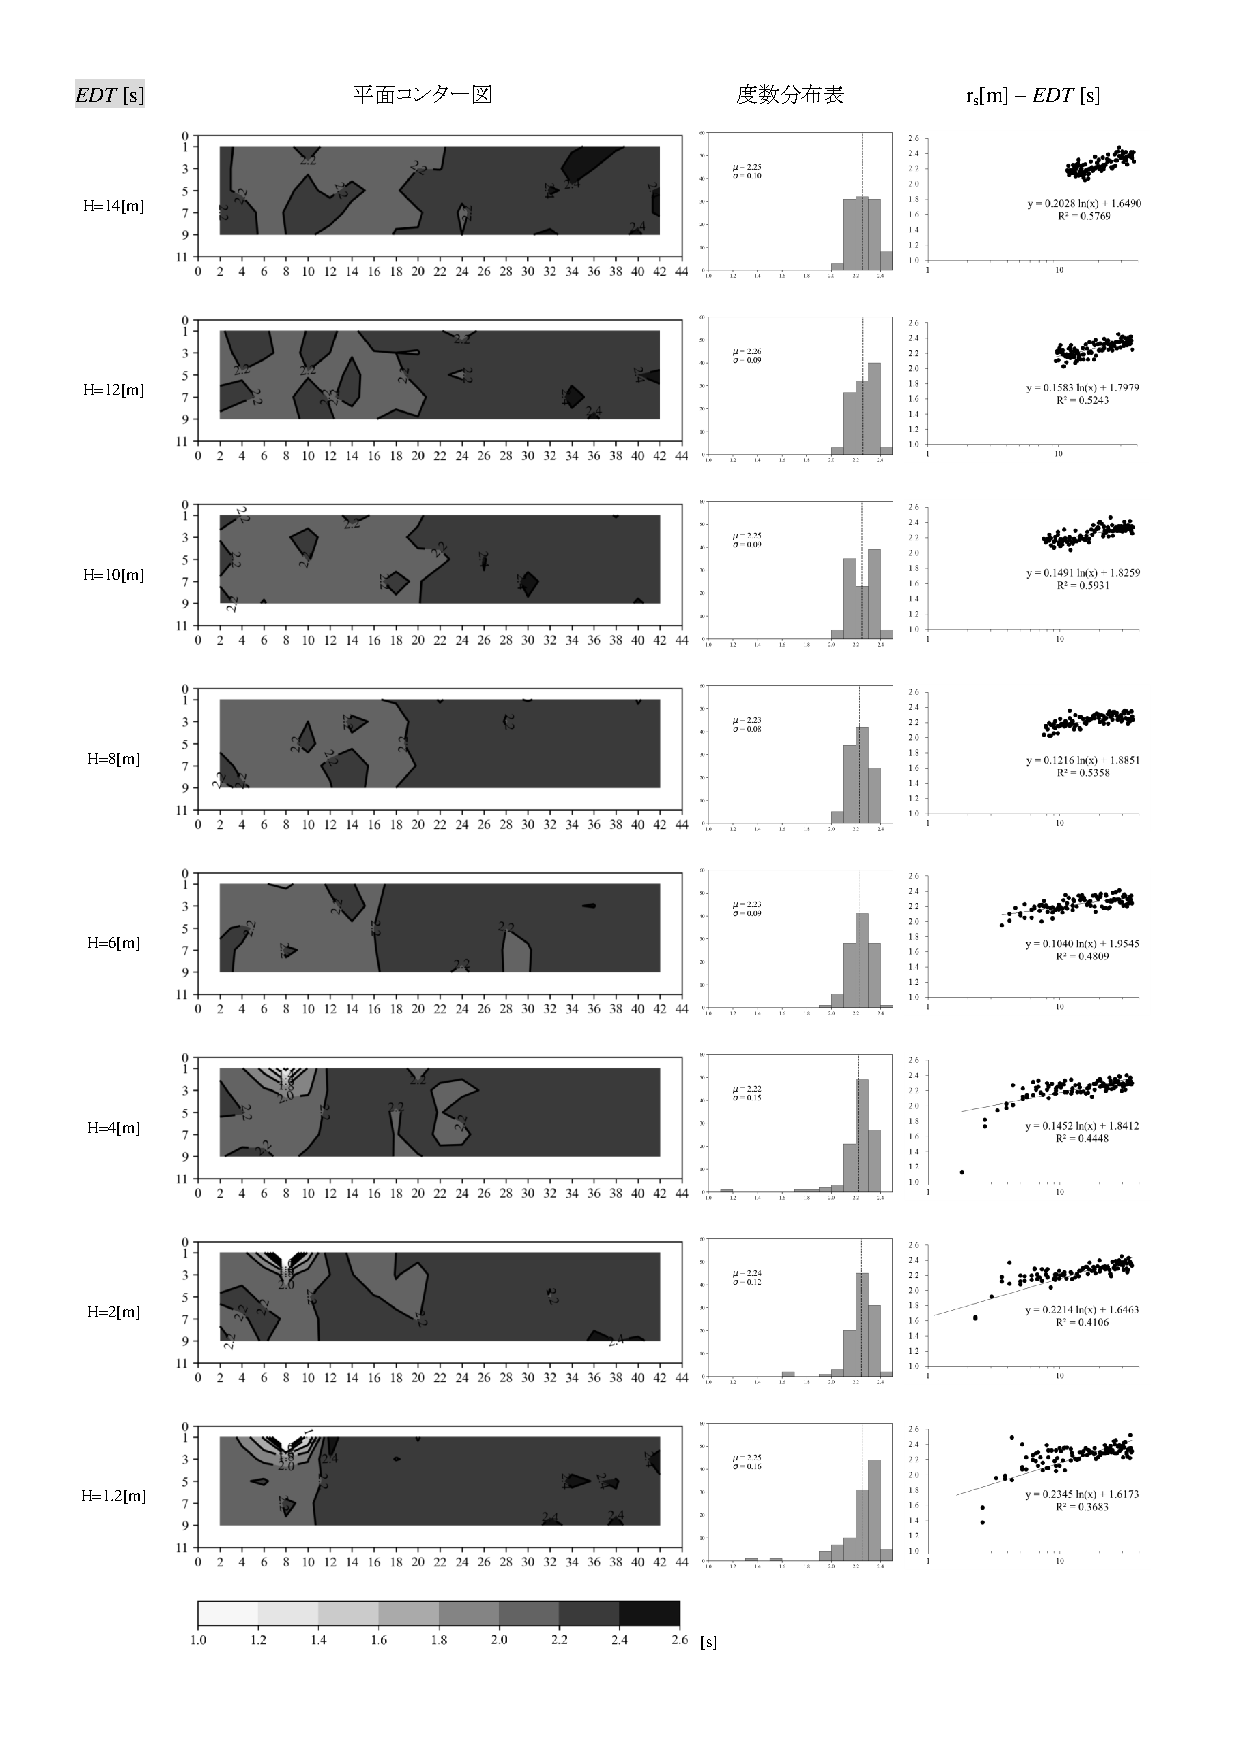
\includegraphics[keepaspectratio,width=1\hsize,angle=0]
                          {04_att/Onkyo_rec4.pdf}
      \end{minipage}
\newpage
      \begin{minipage}{1\hsize}
        \centering
          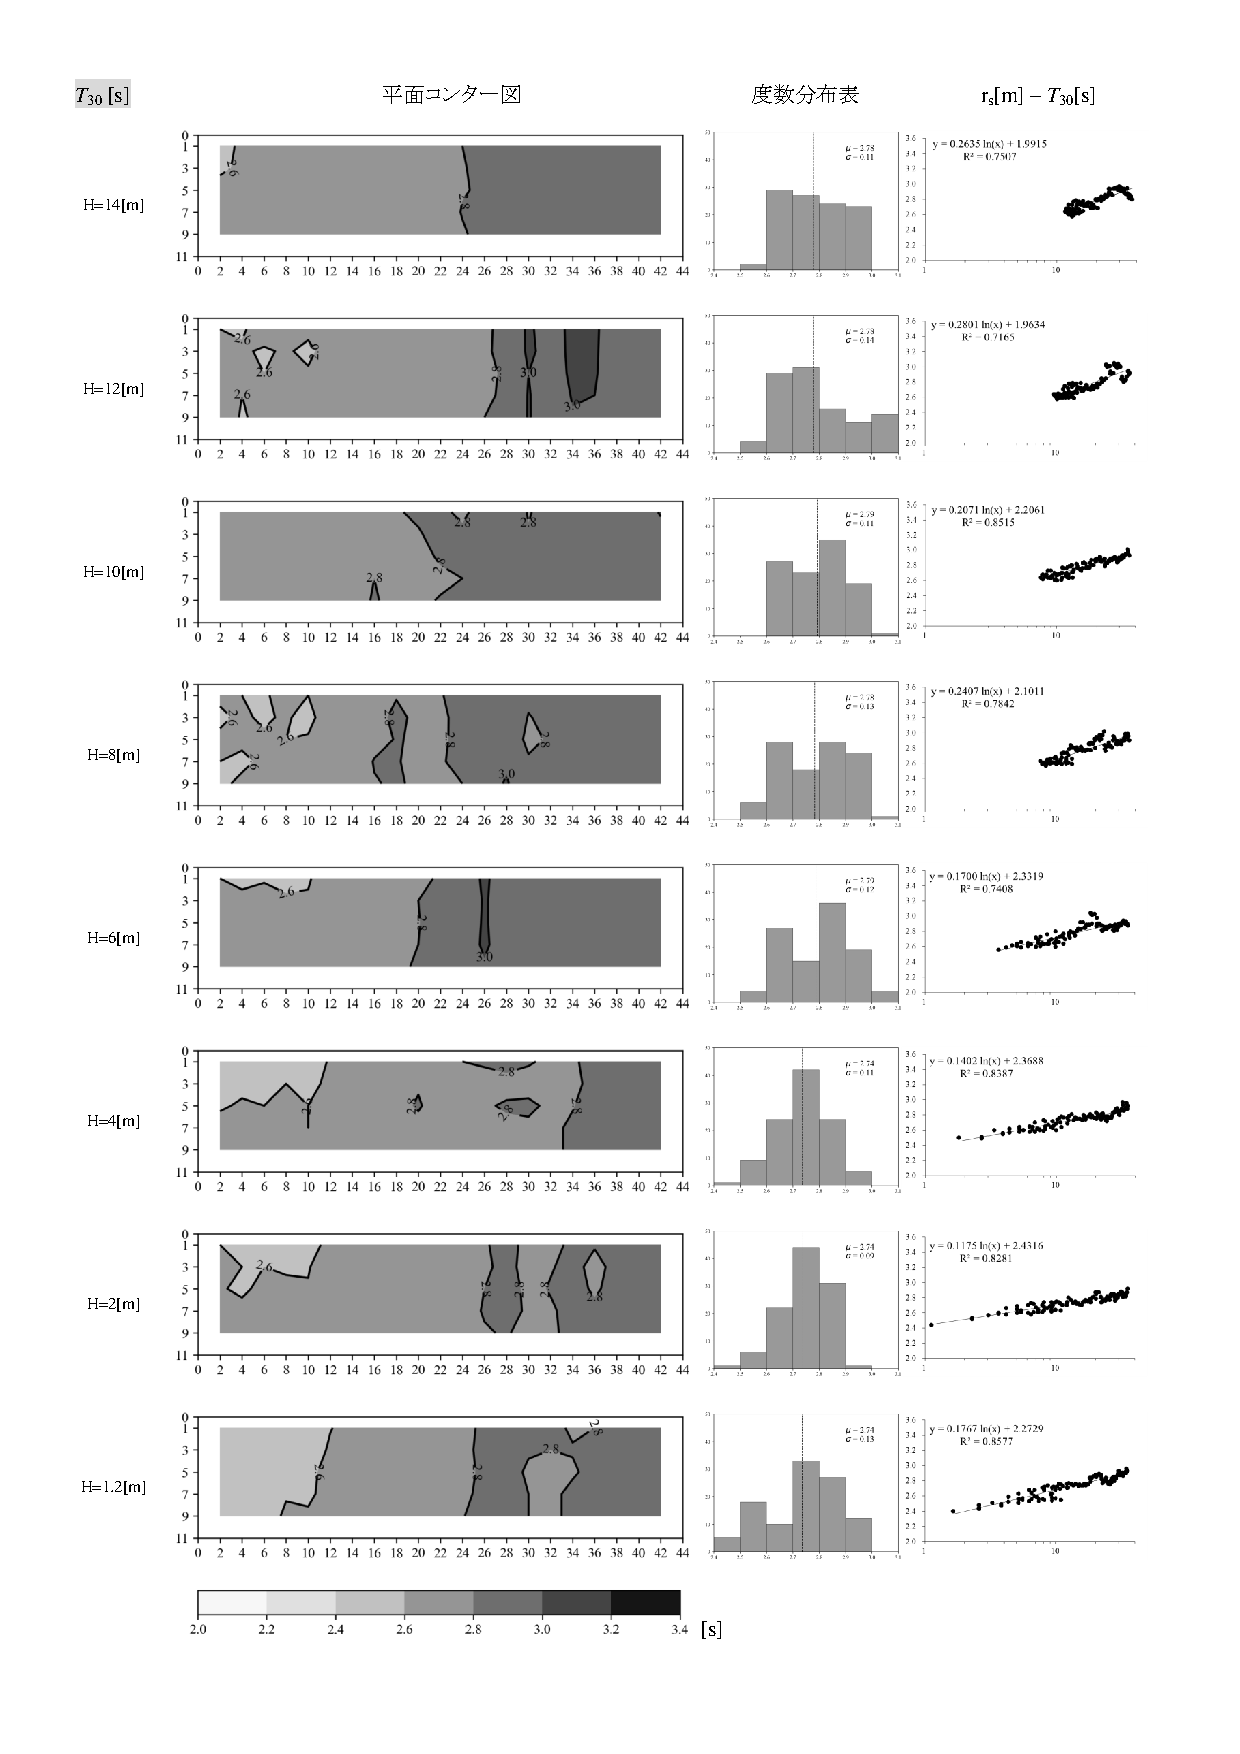
\includegraphics[keepaspectratio,width=1\hsize,angle=0]
                          {04_att/Onkyo_rec5.pdf}
      \end{minipage}
\newpage
      \begin{minipage}{1\hsize}
        \centering
          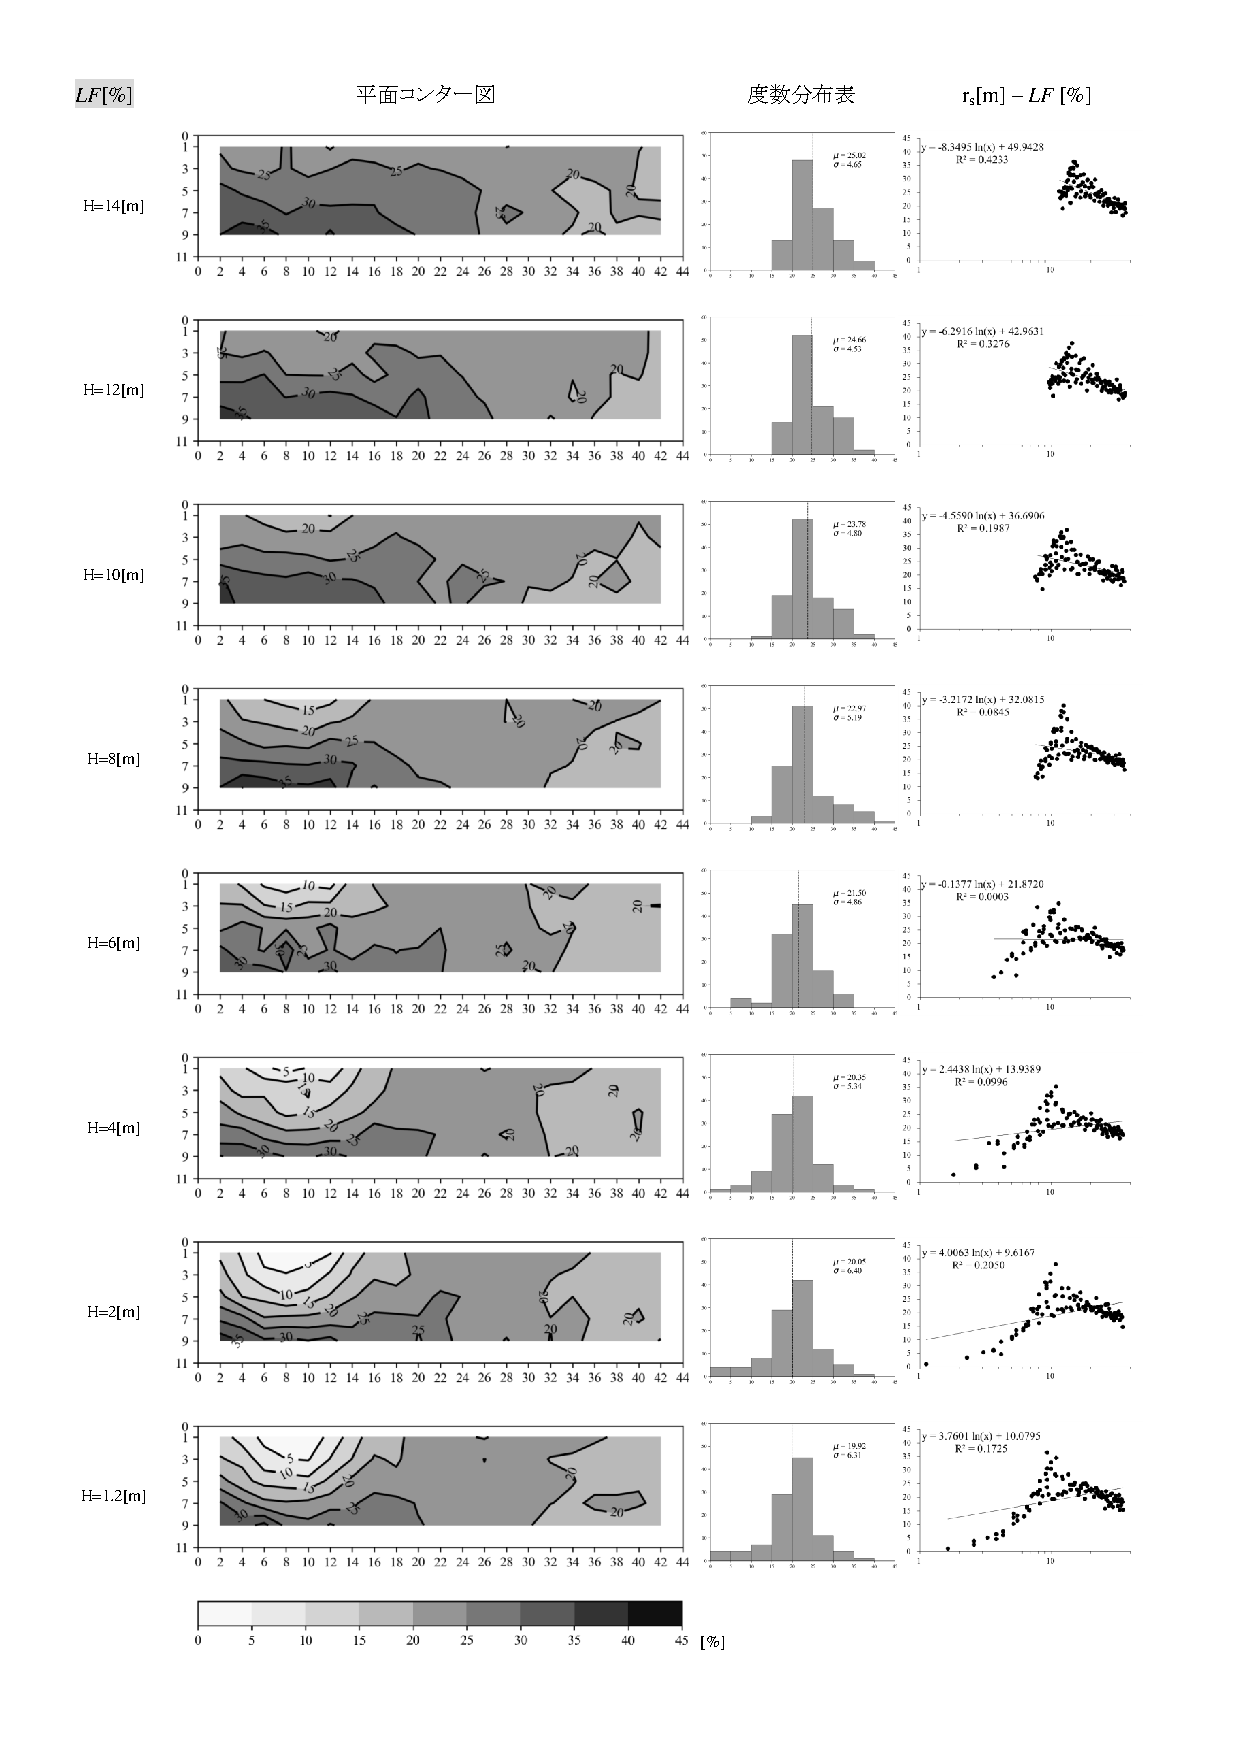
\includegraphics[keepaspectratio,width=1\hsize,angle=0]
                          {04_att/Onkyo_rec6.pdf}
      \end{minipage}      
\newpage
      \begin{minipage}{1\hsize}
        \centering
          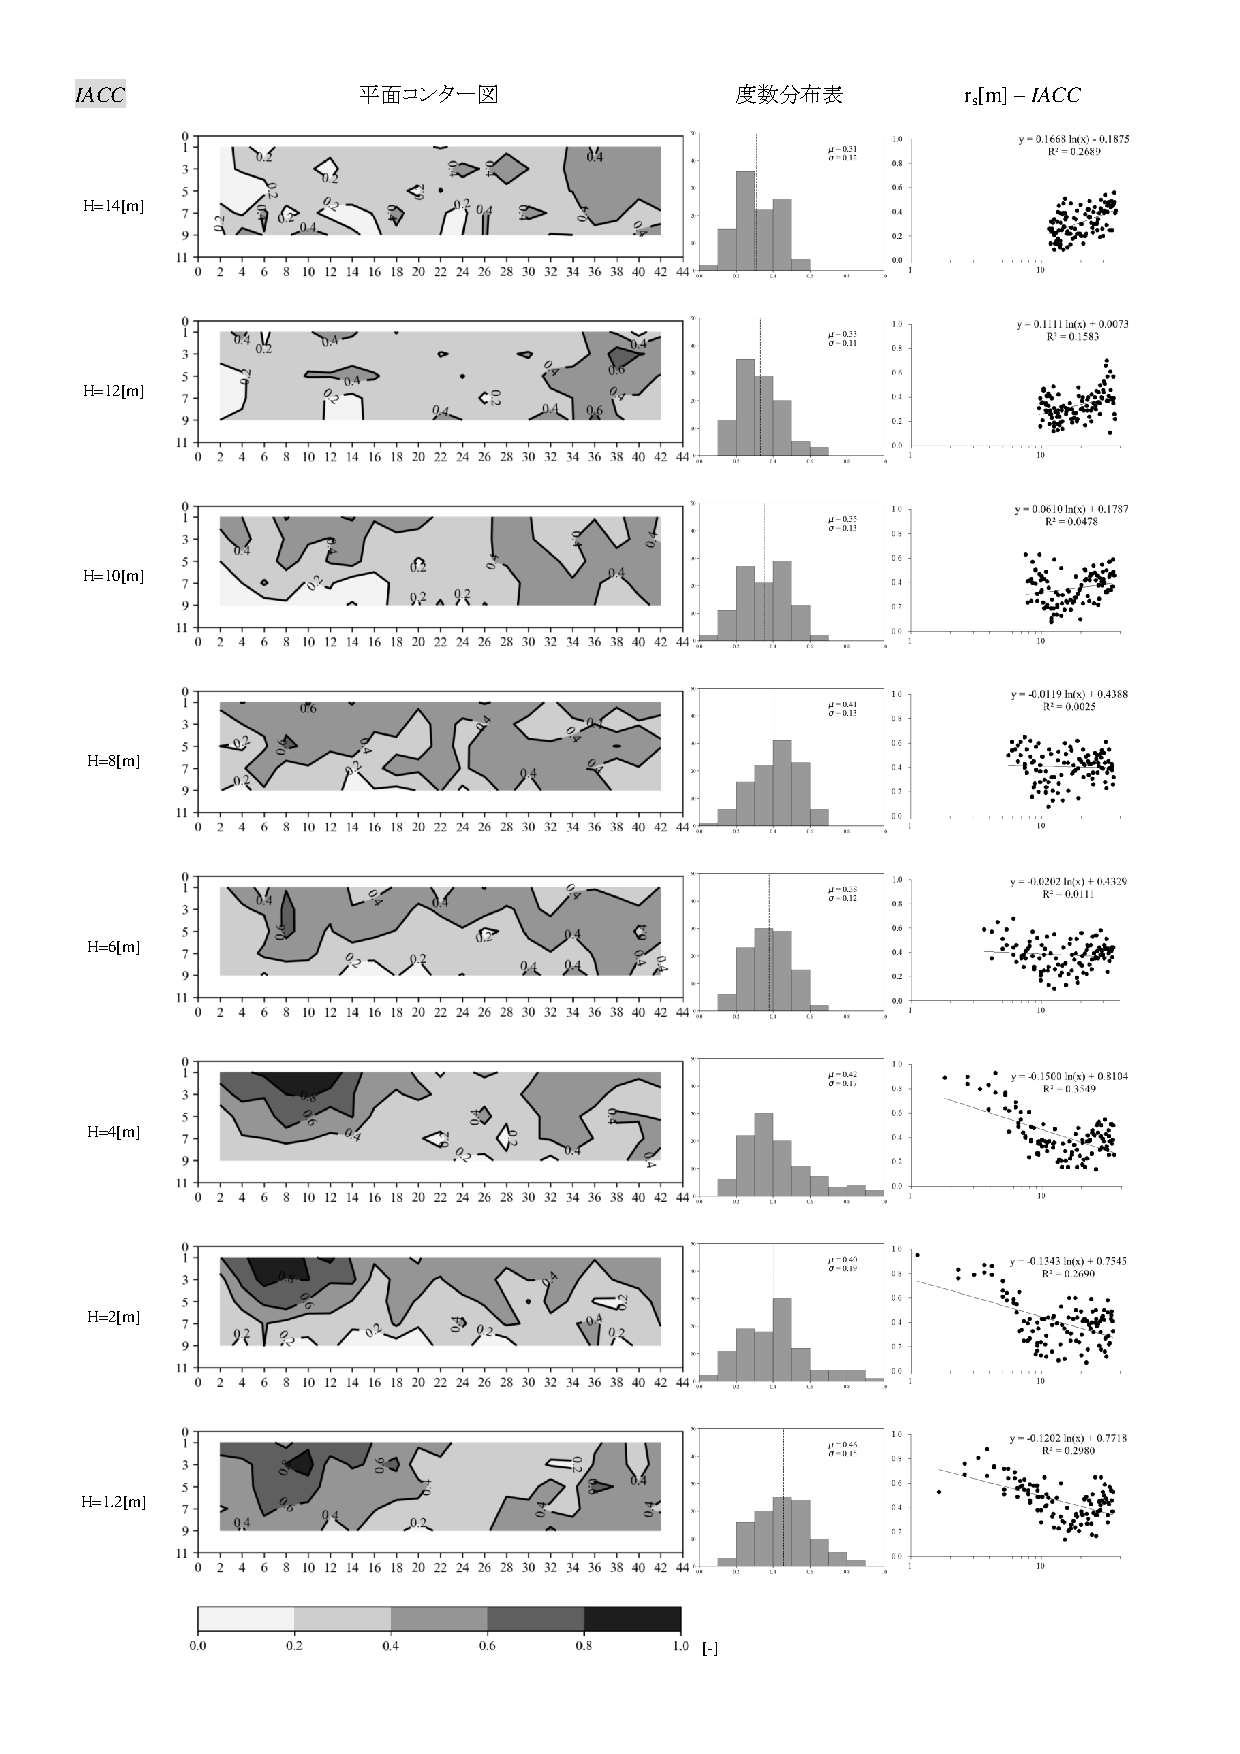
\includegraphics[keepaspectratio,width=1\hsize,angle=0]
                          {04_att/Onkyo_rec7.pdf}
      \end{minipage}      

一元配置分散分析(対応あり)の結果を\tabref{ichigen}に示す。
$EDT$を除く全ての指標値で有意な差が認められた。
次にBonferroniの多重比較を行った結果を示す\tabref{taju}。

\begin{table}[htbp]
\centering
\caption{The result of one-way analysis of variance}
\label{tab:ichigen}
\begin{tabular}{cccccccc}
\hline
\begin{tabular}[c]{@{}c@{}}Acoustic\\ parameter\end{tabular} & \textit{G} & \textit{EDT} & $C_{80}$ & $D_{50}$ & \textit{LF} & \textit{IACC} & $T_{30}$ \\ \hline
judge & ** & n.s. & * & ** & ** & ** & ** \\ \hline
\multicolumn{8}{l}{**:$p$\textless{}0.01, *:$p$\textless{}0.05}
\end{tabular}
\end{table}





\section{残響エネルギ特性}
\section{時間エネルギ特性}
\section{音圧レベル特性}
